% --------------------------------------------------------------------------- %
% Short (8 min) beamer talk -- public health expert audience.                  %
% Restructured from slides/covid_mortality_slides.tex: puzzle-first opening,   %
% compressed model, mechanisms table as the payoff.                            %
% Adapted from the poster poster/covid_mortality.tex                           %
% Compile with: pdflatex (twice) or latexmk -pdf                               %
% --------------------------------------------------------------------------- %
\documentclass[aspectratio=169,10pt]{beamer}

\usetheme{default}
\usecolortheme{default}
\setbeamertemplate{navigation symbols}{}
\setbeamertemplate{itemize items}[circle]
\setbeamertemplate{frametitle}[default][left]

\usepackage[scaled]{helvet}
\renewcommand{\familydefault}{\sfdefault}

\usepackage[T1]{fontenc}
\usepackage[utf8]{inputenc}
\usepackage{graphicx}
\usepackage{amsmath}
\usepackage{booktabs}

%%% Colors taken from the poster %%%%%%%%%%%%%%%%%%%%%%%%%%%%%%%%%%%%%%%%%%%%%%
\definecolor{headerfontcol}{RGB}{190,0,0}   % poster title red
\definecolor{bordercol}{RGB}{105,105,105}

\setbeamercolor{frametitle}{fg=headerfontcol,bg=white}
\setbeamercolor{title}{fg=headerfontcol}
\setbeamercolor{structure}{fg=headerfontcol}
\setbeamercolor{footline}{fg=bordercol}
\setbeamerfont{frametitle}{series=\bfseries}
\setbeamerfont{title}{series=\bfseries}

%%% Slide number only (backup slides must not inflate a total) %%%%%%%%%%%%%%%%%
\setbeamertemplate{footline}{%
  \hfill\usebeamercolor[fg]{footline}%
  \scriptsize\insertframenumber\hspace*{2ex}\vspace*{1ex}%
}

%%% Figures live next to the poster %%%%%%%%%%%%%%%%%%%%%%%%%%%%%%%%%%%%%%%%%%%
\graphicspath{{./}{images/}{../poster/}{../poster/images/}}

\newcommand{\compresslist}{%
  \setlength{\itemsep}{3pt}%
  \setlength{\parskip}{0pt}%
  \setlength{\parsep}{0pt}%
}
\newcommand{\figcaption}[1]{{\tiny #1}}
\newcommand{\punch}[1]{{\color{headerfontcol}\bfseries #1}}

%%%%%%%%%%%%%%%%%%%%%%%%%%%%%%%%%%%%%%%%%%%%%%%%%%%%%%%%%%%%%%%%%%%%%%%%%%%%%%%
\title{\large COVID-19 disrupted patterns of cause-specific mortality in Switzerland}
\author{\small Anthony Hauser\inst{1} \and Moritz Wagner\inst{2} \and Anna Fesser\inst{2} \and
  Karim Abawi\inst{3} \and Anne Laube\inst{2} \and Garyfallos Konstantinoudis\inst{4} \and
  Julien Riou\inst{1}}
\institute{\scriptsize
  \inst{1} Unisant\'e, University of Lausanne \quad
  \inst{2} Federal Statistical Office \quad
  \inst{3} Federal Office of Public Health \quad
  \inst{4} Imperial College London}
\date{\small\today}

%%% Published reference for this work %%%%%%%%%%%%%%%%%%%%%%%%%%%%%%%%%%%%%%%%%
% TODO: add the volume number once confirmed on the journal page.
\newcommand{\thispaper}{Hauser A, Wagner M, Fesser A, Abawi K, Laube A,
  Konstantinoudis G, Riou J. \emph{COVID-19 disrupted patterns of cause-specific
  mortality in Switzerland.} Int J Public Health 2026;1609856.
  doi:10.3389/ijph.2026.1609856}

%%%%%%%%%%%%%%%%%%%%%%%%%%%%%%%%%%%%%%%%%%%%%%%%%%%%%%%%%%%%%%%%%%%%%%%%%%%%%%%
\begin{document}

% cumulative ~0:20
\begin{frame}[plain]
  \titlepage
  \vspace{-1em}
  \begin{center}\scriptsize\color{bordercol}
    Published in the \emph{International Journal of Public Health} (2026) ---
    doi:10.3389/ijph.2026.1609856
  \end{center}
\end{frame}

%%% 0. THE HOOK: one death, one line %%%%%%%%%%%%%%%%%%%%%%%%%%%%%%%%%%%%%%%%%
% cumulative ~0:50
\begin{frame}{One death, several causes}
  \begin{center}
    \begin{minipage}{0.72\linewidth}
      \setlength{\fboxsep}{10pt}%
      \fcolorbox{bordercol}{white}{\begin{minipage}{\linewidth}
        \small An 85-year-old man, November 2020:\\[0.4em]
        \begin{tabular}{@{}ll@{}}
          Immediate cause    & respiratory failure \\
          Underlying cause   & \textbf{COVID-19?} \quad \textbf{heart failure?} \\
          Contributing       & dementia, hypertension \\
        \end{tabular}
      \end{minipage}}
    \end{minipage}
  \end{center}
  \vspace{0.6em}
  \begin{itemize}\compresslist
    \item National mortality statistics keep \textbf{one} cause per death ---
          the underlying one.
    \item In a pandemic, which line is chosen shifts for reasons unrelated to
          the patient: testing, awareness, certification practice.
  \end{itemize}
  \vspace{0.3em}
  \begin{center}
    \punch{So causes of death stop being independent ---\\
    and so do their excesses.}
  \end{center}
\end{frame}

%%% 1. FROM THE PREVIOUS PROJECT TO THIS ONE -- framing only %%%%%%%%%%%%%%%%%
% cumulative ~1:40
\begin{frame}{Where we come from}
  \textbf{Previous project}\footnote[frame]{\tiny Riou J, Hauser A, Fesser A,
    Althaus CL, Egger M, Konstantinoudis G. \emph{Direct and indirect effects of
    the COVID-19 pandemic on mortality in Switzerland.} Nat Commun 2023;14:90.}:
  partition \textbf{all-cause} mortality into deaths directly attributable to
  SARS-CoV-2 and deaths indirectly attributable to the pandemic.
  \begin{itemize}\compresslist
    \item Laboratory-confirmed deaths \textbf{underestimate} COVID-19 mortality
          (by a factor of 0.72, 95\% credible interval [CrI] 0.46--0.78).
    \item Net of COVID-19 deaths, mortality was \textbf{lower} than expected
          ($-4\%$, 95\% CrI $-8$ to $0$) --- an indirect \emph{beneficial} effect,
          attributed to restriction measures and to mortality displacement
          (``harvesting'').
  \end{itemize}
  \vfill
  \textbf{But this was all-cause: the mechanisms were inferred, not observed.}
  \vfill
  \begin{center}
    \punch{Can we identify the deaths that should have been attributed to COVID-19?}\\[0.2em]
    \punch{What were the indirect effects of the pandemic on the different causes of death?}
  \end{center}
  \vfill
\end{frame}

%%% 2. WHY CAUSES MUST BE MODELLED JOINTLY %%%%%%%%%%%%%%%%%%%%%%%%%%%%%%%%%%%%
% cumulative ~2:30
\begin{frame}{Why cause-specific is not enough}
  Going cause by cause does not answer either question:
  \begin{itemize}\compresslist
    \item a \textbf{deficit} in one cause may be a real decrease, or deaths
          reallocated to COVID-19 --- indistinguishable within a single cause;
    \item an \textbf{excess} in one cause may be a delayed effect of infection,
          or an unascertained COVID-19 death.
  \end{itemize}
  \vfill
  \begin{center}
    The information that separates them lies \punch{between} causes:\\
    which causes move together, and \punch{with what delay}.
  \end{center}
  \vfill
  \textbf{Approach:} a Bayesian \textbf{multivariate} model of weekly
  cause-specific mortality, estimating excess mortality for all causes jointly
  together with their dependence structure.
  \vspace{0.3em}

  {\scriptsize\color{bordercol} Related Swiss work analyses causes
  \emph{separately}: the FSO documents shifts in the distribution of causes, and
  Dur\'an et al.\ (Ann Epidemiol 2025) compare underlying vs multiple causes
  monthly, by broad group. Here the temporal dynamics of causes are modelled
  \emph{jointly}.}
\end{frame}

%%% 2. THE HEADLINE %%%%%%%%%%%%%%%%%%%%%%%%%%%%%%%%%%%%%%%%%%%%%%%%%%%%%%%%%%%
% cumulative ~3:20
\begin{frame}{Result 1: the previous finding, now week by week}
  \begin{columns}[t]
    \begin{column}{0.55\linewidth}
      \centering
      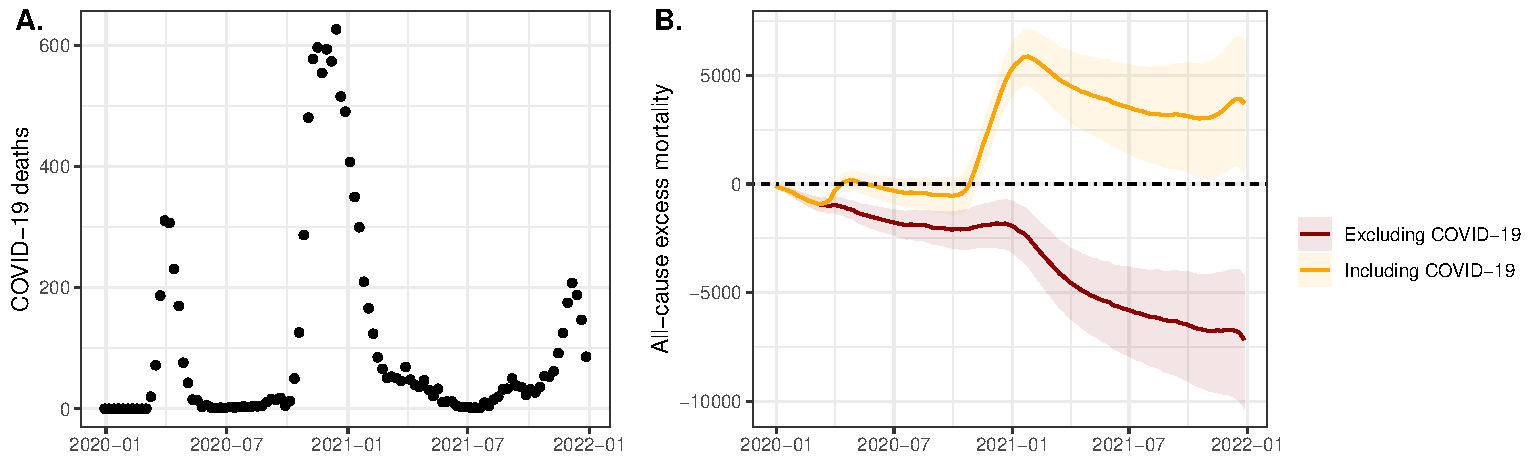
\includegraphics[width=\linewidth,height=0.72\textheight,keepaspectratio]{fig2_v2.pdf}\\[0.2em]
      \figcaption{\textbf{Figure 1.} A. Weekly COVID-19 deaths in 80+.
        B. Excess mortality with and without COVID-19 in 80+.}
    \end{column}
    \begin{column}{0.43\linewidth}
      \vspace{1em}
      \begin{itemize}\compresslist
        \item Sharp rise in cumulative excess during major waves, then a
              \textbf{deficit} in the following weeks.
        \item \punch{The all-cause deficit is reproduced here, and
              resolved in time:} excess and deficit alternate around waves.
      \end{itemize}
      \vspace{0.5em}
      \begin{center}
        Deficits and excesses are not independent across causes.
      \end{center}
    \end{column}
  \end{columns}
\end{frame}

%%% 3. METHOD -- one slide, correlation is the point %%%%%%%%%%%%%%%%%%%%%%%%%%%
% cumulative ~4:10
\begin{frame}{A multivariate model, in one slide}
  Weekly deaths by cause $i$, region $r$, sex $s$, age group; 2011--2019 as the
  baseline, 9 cause groups (ICD-10, immediate + underlying + contributing).
  \[
    y_{irs}(t) \sim \text{Poisson}(\mu_{irs}(t)), \qquad
    \log \mu_{irs}(t) = \alpha_i + \beta_{ir} + \gamma_{is}
      + f_{i}(t) + g_{i}(t) + \varepsilon_i(t) + \log N_{rst}
  \]
  with long-term and seasonal trends $f_i,g_i$ (Gaussian processes) and
  \[
    \varepsilon(t) \sim \mathcal{N}(0,\Sigma), \qquad
    E_{irs}(t) := y_{irs}(t) - \tilde{y}_{irs}(t).
  \]
  \vspace{-0.4em}
  \begin{itemize}\compresslist
    \item \punch{$\Sigma$ is not a nuisance --- it is the scientific quantity.}
          Cross-cause dependence is estimated, not assumed.
    \item Excess mortality is obtained \emph{jointly} for all causes, so
          excesses and deficits can be compared and correlated.
  \end{itemize}
\end{frame}

%%% 4. RESULT: WHAT MOVED, AND WHEN %%%%%%%%%%%%%%%%%%%%%%%%%%%%%%%%%%%%%%%%%%%
% cumulative ~5:20
\begin{frame}{Result 2: what moved, and when}
  \begin{columns}[t]
    \begin{column}{0.44\linewidth}
      \vspace{0.5em}
      \begin{itemize}\compresslist
        \item CVD excess concentrates \emph{during} the waves, followed by
              deficits.
        \item Mental/neurological: strong decrease, largest in the Alpha wave.
        \item Cancer: deficit mainly during the Alpha wave.
        \item Respiratory (non-COVID): \textbf{consistently} below expected at
              all ages, larger deficits at older ages.
      \end{itemize}
    \end{column}
    \begin{column}{0.54\linewidth}
      \centering
      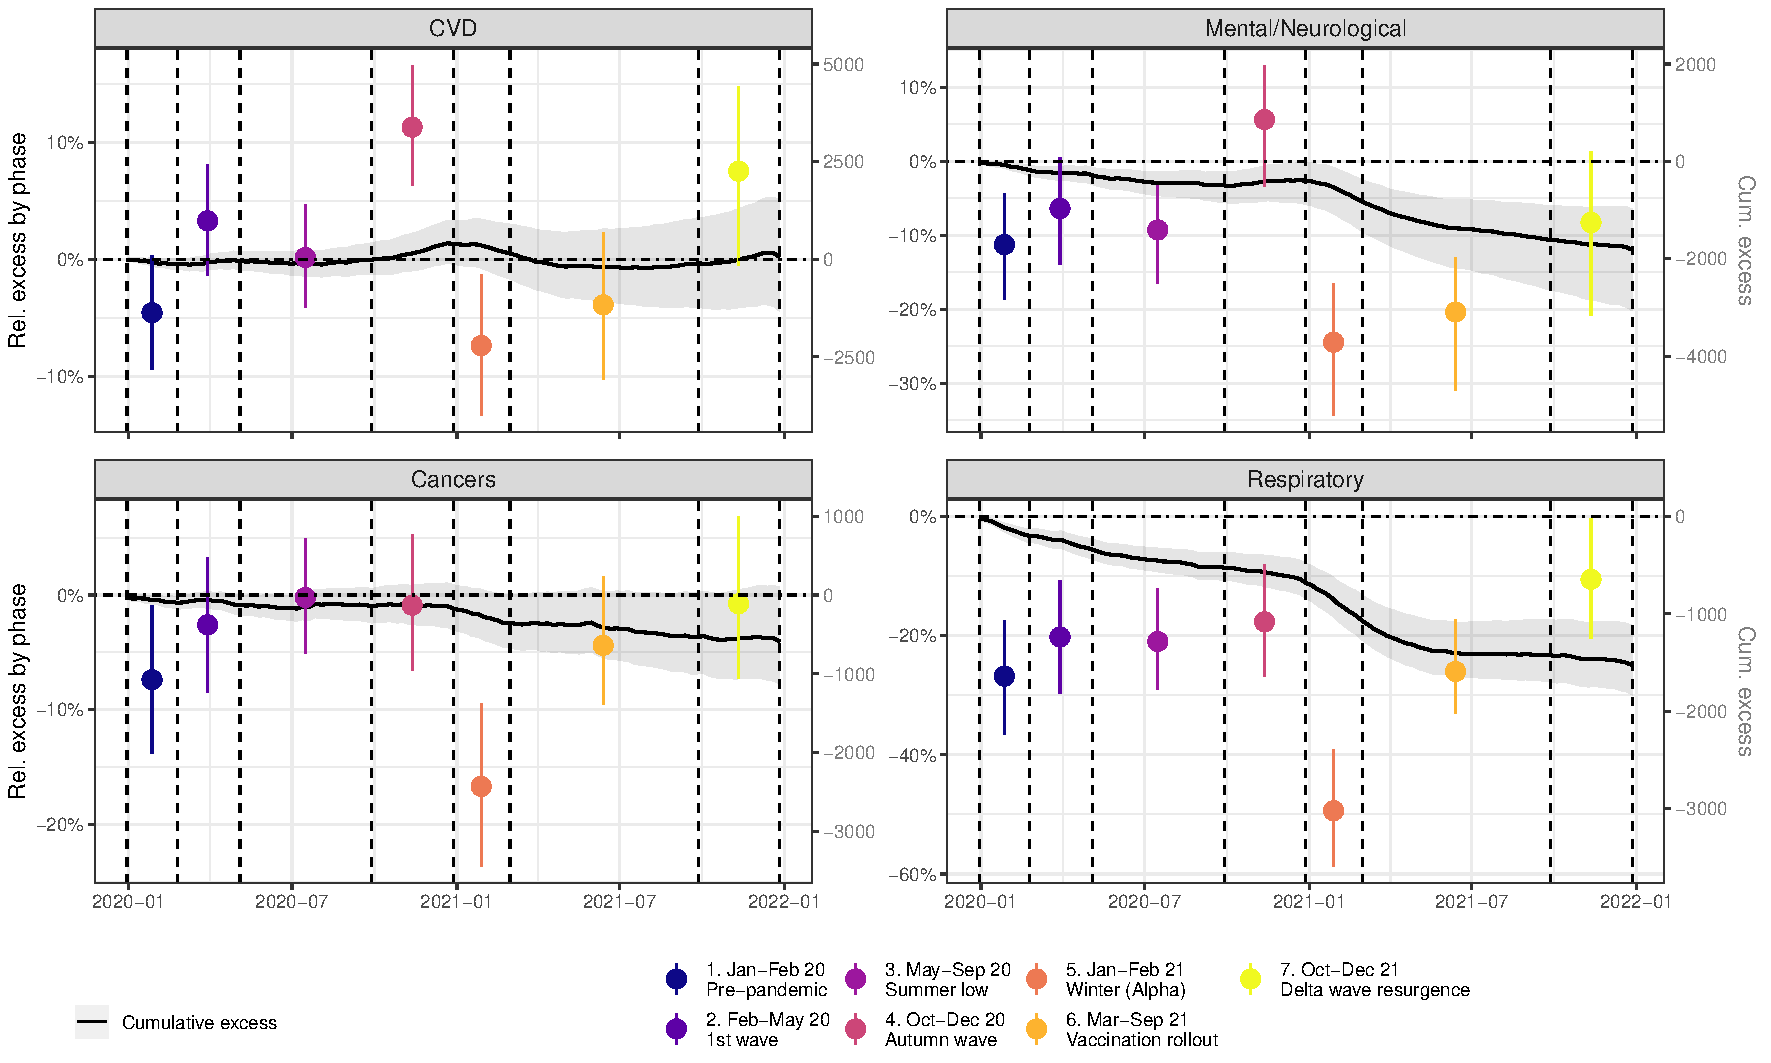
\includegraphics[width=\linewidth,height=0.74\textheight,keepaspectratio]{fig3_v2.pdf}\\[0.2em]
      \figcaption{\textbf{Figure 2. Cause-specific excess mortality by phase, 80+.}
        Black: cumulative excess in 2020--21 (95\% CrI in gray).
        Colored points/bars: phase-specific relative excess (95\% CrI).}
    \end{column}
  \end{columns}
\end{frame}

%%% 5. RESULT: LAGS GIVE MECHANISM %%%%%%%%%%%%%%%%%%%%%%%%%%%%%%%%%%%%%%%%%%%%
% cumulative ~6:30
\begin{frame}{Result 3: lags turn pattern into mechanism}
  \begin{columns}[t]
    \begin{column}{0.45\linewidth}
      \vspace{0.5em}
      \begin{itemize}\compresslist
        \item Partial correlations up to $\sim 0.5$ between COVID-19 excess and
              excess from CVD and mental/neurological causes.
        \item Similar for other respiratory diseases.
        \item \punch{Correlations peak at lags of 1--3 weeks} --- COVID-19 excess
              deaths occur slightly \emph{after} the CVD and mental/neurological
              ones.
        \item Cancer: weak or negative correlation with COVID-19.
      \end{itemize}
      \vspace{0.3em}
      {\footnotesize\punch{Why the lag matters:} COVID-19 excess comes
      \emph{after} the CVD and mental/neurological excess. Delayed complications
      of infection would put the other causes \emph{after} COVID-19, not before
      --- so the ordering argues for unascertained COVID-19 deaths early in the
      waves rather than for delayed effects.}
    \end{column}
    \begin{column}{0.53\linewidth}
      \centering
      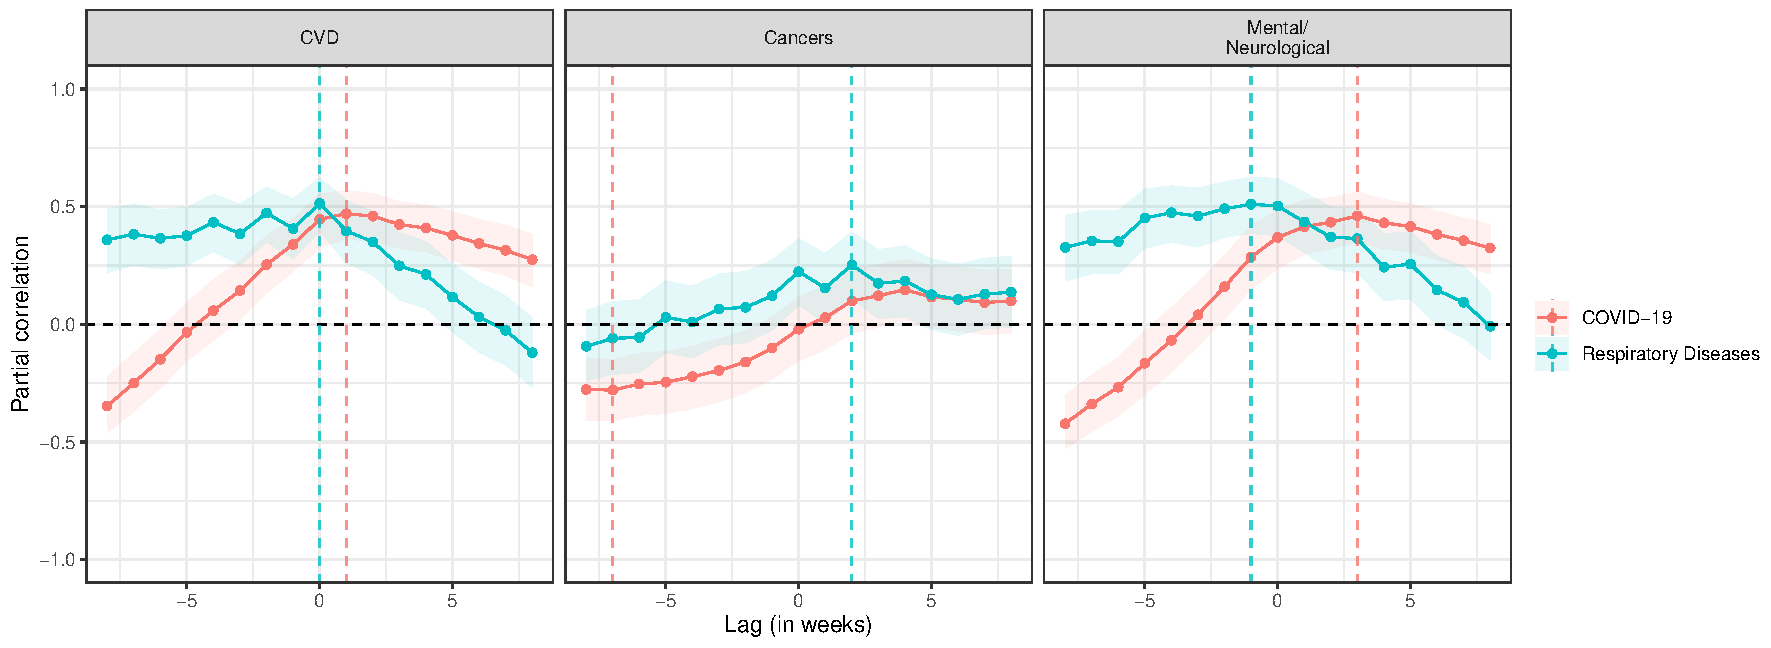
\includegraphics[width=\linewidth,height=0.74\textheight,keepaspectratio]{fig4_v2.pdf}\\[0.2em]
      \figcaption{\textbf{Figure 3.} Partial correlation between excess mortality
        from COVID-19 (red) or other respiratory diseases (blue) and excess
        mortality from CVD, cancers or mental/neurological diseases, 80+.}
    \end{column}
  \end{columns}
\end{frame}

%%% 6. PUZZLE RESOLVED %%%%%%%%%%%%%%%%%%%%%%%%%%%%%%%%%%%%%%%%%%%%%%%%%%%%%%%%
% cumulative ~7:20
\begin{frame}{Result 4: the cancer deficit, checked directly}
  \vfill
  The cancer deficit is the cleanest test of the question we opened with.
  Checked independently with \textbf{multiple-cause-of-death} data:
  \begin{itemize}\compresslist
    \item Total deaths \emph{with} cancer did \textbf{not} decline in
          January--February 2021 --- a slight increase in 65--79, larger in 80+.
    \item The largest increase was for \textbf{high-survival} cancers,
          particularly in the 80+.
  \end{itemize}
  \vfill
  \begin{center}
    \punch{Cancer patients did not stop dying --- they died \emph{of} COVID-19.}\\[0.3em]
    A reallocation between causes, not a drop in cancer mortality.
  \end{center}
  \vfill
\end{frame}

%%% 7. THE PAYOFF %%%%%%%%%%%%%%%%%%%%%%%%%%%%%%%%%%%%%%%%%%%%%%%%%%%%%%%%%%%%%
% cumulative ~8:00
\begin{frame}{Four mechanisms explain the disruptions}
  \centering
  {\scriptsize
  \begin{tabular}{p{2.4cm} p{4.2cm} p{5.2cm}}
    \toprule
    \textbf{Mechanism} & \textbf{Explanation} & \textbf{Evidence here} \\
    \midrule
    \raggedright Under-ascertainment of COVID-19 deaths &
      Infections not identified at death inflated other causes. &
      CVD excess in autumn 2020 aligned with COVID-19 mortality; short lags. \\
    \midrule
    \raggedright Delayed SARS-CoV-2 effects &
      Post-infection complications raise death risk weeks to months later. &
      Low evidence for Switzerland. \\
    \midrule
    \raggedright Mortality displacement &
      Early deaths among frail individuals create later deficits. &
      Deficits in dementia and CVD after the autumn 2020 wave; cancer patients
      dying from COVID-19. \\
    \midrule
    \raggedright Pandemic response (NPIs) &
      Control measures reduced circulation of respiratory pathogens. &
      Large decrease in non-COVID respiratory mortality; lower winter mortality
      in older adults. \\
    \bottomrule
  \end{tabular}}
\end{frame}

%%% 8. TAKE-HOME %%%%%%%%%%%%%%%%%%%%%%%%%%%%%%%%%%%%%%%%%%%%%%%%%%%%%%%%%%%%%%
% cumulative ~8:30
\begin{frame}{Take-home}
  \begin{enumerate}\compresslist
    \item Cause-specific excess mortality is \textbf{not nine separate problems} ---
          it is one coupled system, and modelling it jointly is what makes the
          causes interpretable.
    \item Net of COVID-19 deaths, Swiss mortality was \textbf{below} expectation
          in 2020--21.
    \item Deficits are largely \textbf{reallocation and displacement}, not lives
          saved --- except for respiratory mortality, where the NPI effect looks real.
  \end{enumerate}
  \vfill
  \begin{center}
    {\scriptsize\thispaper}\\[0.6em]
    \small anthony.hauser@unisante.ch
  \end{center}
\end{frame}

%%% BACKUP %%%%%%%%%%%%%%%%%%%%%%%%%%%%%%%%%%%%%%%%%%%%%%%%%%%%%%%%%%%%%%%%%%%%
\appendix

\begin{frame}[plain]
  \centering\vfill{\Large\bfseries\color{headerfontcol} Backup slides}\vfill
\end{frame}

\begin{frame}{Backup: model fit and cross-cause patterns, 80+}
  \centering
  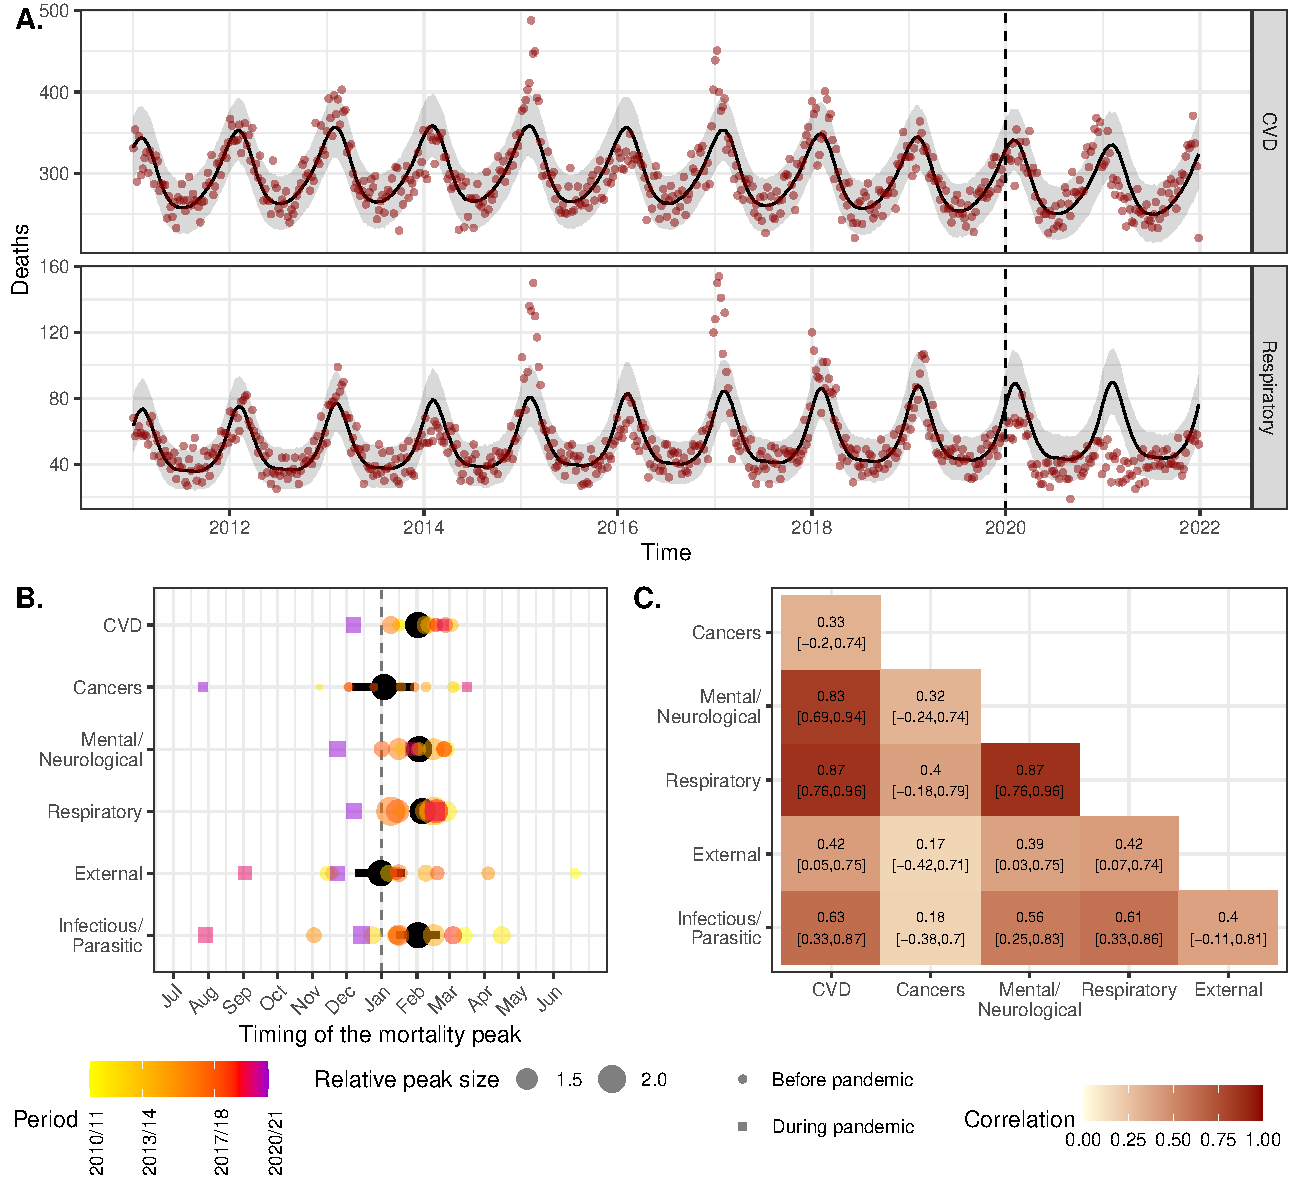
\includegraphics[width=0.88\linewidth,height=0.78\textheight,keepaspectratio]{fig1_v4.pdf}\\[0.2em]
  \figcaption{A. Weekly deaths observed (red) and model estimates/predictions
    (black) with 95\% CrI (gray). B. Timing of mortality peaks; colored points:
    observed, black: posterior estimate with 95\% CrI.
    C. Cross-cause correlation of excess mortality.}
\end{frame}

\begin{frame}{Backup: data and cause groups}
  \begin{itemize}\compresslist
    \item Deaths $y_{irs}(t)$ by cause, sex, NUTS-2 region, year and week; age
          groups 0--17, 18--39, 40--64, 65--79, 80+; 2011--2021.
    \item \textbf{Underlying} cause of death (ICD-10), grouped into 9 categories:
          cardiovascular, mental/neurological, respiratory, infectious, cancer,
          external, suicide, COVID-19, other. Multiple causes are used only in
          the supplementary cancer analysis.
    \item Population $N_{rst}$ by age, sex, region; weekly linear interpolation.
    \item Baseline fitted on 2011--2019; 2020--21 predicted out of sample.
  \end{itemize}
\end{frame}

\begin{frame}{Backup: what the correlations can and cannot show}
  \textbf{Certificate competition is not the threat.} If a death is coded
  COVID-19 \emph{instead of} CVD, COVID-19 rises while CVD falls: that pushes the
  correlation \textbf{negative}. The observed correlations are positive, so this
  mechanism works against what we see rather than creating it.
  \vspace{0.5em}

  \textbf{What does create a positive correlation:}
  \begin{itemize}\compresslist
    \item \textbf{Under-ascertainment} --- a COVID-19 death never identified,
          added to CVD: both series rise together during waves.
    \item \textbf{Genuine triggered deaths} --- infection causing cardiovascular
          death.
  \end{itemize}
  \vspace{0.3em}
  \punch{The correlation alone does not separate these two.} Both are positive
  and both act at short lag. We report under-ascertainment as one of four
  mechanisms rather than claiming to have isolated it.
  \vspace{0.5em}

  \textbf{Note:} mortality displacement is evidenced by the \emph{phase-specific}
  excess --- deficits following waves --- not by the correlation structure.
\end{frame}

\begin{frame}{Backup: is this just harvesting?}
  \begin{itemize}\compresslist
    \item Displacement is one of four mechanisms, and the model separates it
          from the others by \emph{timing}:
      \begin{itemize}\compresslist
        \item under-ascertainment $\Rightarrow$ excess in another cause at or
              just \emph{before} the COVID-19 excess,
        \item delayed effects $\Rightarrow$ excess \emph{after} the COVID-19 excess,
        \item displacement $\Rightarrow$ deficit \emph{after} the wave.
      \end{itemize}
    \item Displacement is read off the \textbf{phase-specific} excess (deficit
          after a wave), independently of the correlation structure.
    \item The cancer result is checked with multiple-cause data, which does not
          rely on the underlying-cause assignment at all.
    \item Respiratory deficits persist across the whole period, not only after
          waves --- inconsistent with displacement, consistent with NPIs.
  \end{itemize}
\end{frame}

\end{document}
